\chapter{Precision Systems}
	This chapter is focused on system-related aspects that are relevant to \de{precision systems}, in particular related to the abbe, sine and cosine errors, the kinematic design and the flexure hinges.
	
\section{Alignment: Abbe, sine and cosine errors}
	
	Alignment errors are arising every time we need to align a measurement system and the subject of study: we have to be aware of this kind of error in order to detect them and control/reduce them. In particular the \de{Abbe} error arise every time there's an offset between the object to be measured and the system that perform the measure.
	
	Doing a low-volume production (or with high added value products) it's possible to rely on a manual inspection held by highly trained technician in order to ensure a certain level of quality; considering instead a mass production a handmade check of each component it's not possible due to a fully automated manufacturing and assembly for which there is a little space for adjustment: repeatability and precision must be designed into the product in order to have a high quality.
	
	\paragraph{Abbe's error} Common alignment errors are related to the \textbf{Abbe's error} associated  to it's principle stating that \textit{"the measurement line shall be collinear with the line of motion"}.
	
	\begin{SCfigure}[1][bht]
		\centering
		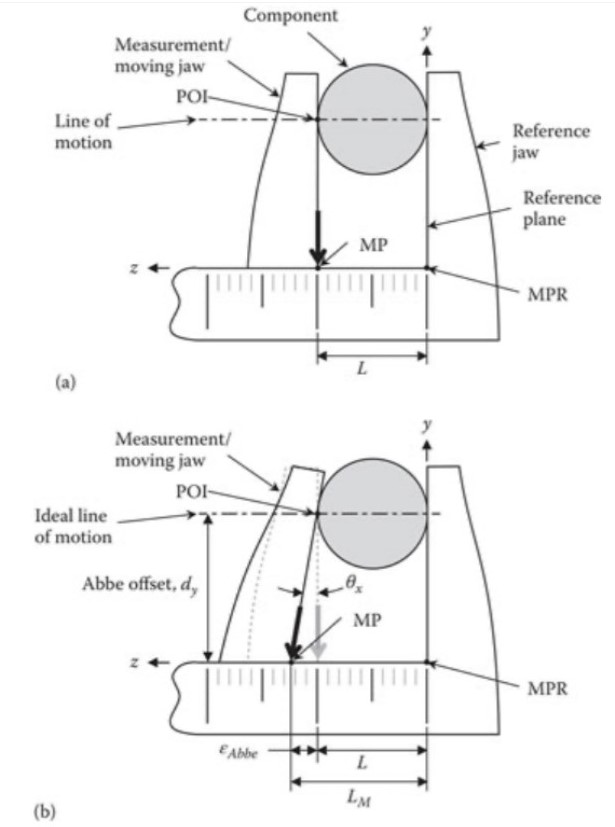
\includegraphics[width=6cm]{abbe-scheme}
		\caption{scheme used to understand the Abbe's error on a calliper. $(a)$ is a correct calliper while $(b)$ is affected by the error.} \label{fig:ps:abbescheme}
	\end{SCfigure}
	An example of this error can be seen in the calliper as in figure \ref{fig:ps:abbescheme}, where the goal is to measure the \textbf{Point of Interest} POI by reading the \textbf{Measurement Point} MP in respect to the Measurement Point \textbf{Reference} MPR. \\
	At a nominal level the two jaws of the calliper should be parallel, and so the point of interest is measured by only looking at the measurement point, but in reality misalignment are always present: this introduce an error $\abbe$ of the measurement point respect to the point of interest. Related to this error we can compute a linear relation but also an expression considering a second order term (that for low error alignment value $\theta_x$ can be neglected), obtaining
	\begin{equation}
		\abbe = d_y \tan\theta_x - \underbrace{L \left(\frac 1 {\cos\theta_x} - 1\right)}_\textrm{2nd ord. term}
	\end{equation}
	
	In reality things are even more complicated: Abbe's error are related to two angle in the 3D space, the so called \textbf{pitch} and \textbf{yaw}
	\begin{equation}
	\begin{split}		
		\abbe & = d_y \tan\theta_x - L \left(\frac 1 {\cos\theta_x} - 1\right) + d_x \tan\theta_y - L \left(\frac 1 {\cos\theta_y} - 1\right) \\
		& = d_y \tan\theta_x + d_x\tan\theta_y - L\left( \frac 1 {\cos\theta_x} + \frac 1 {\cos\theta_y} - 2 \right)
	\end{split}
	\end{equation}
	
	\begin{SCfigure}[2][bht]
		\centering
		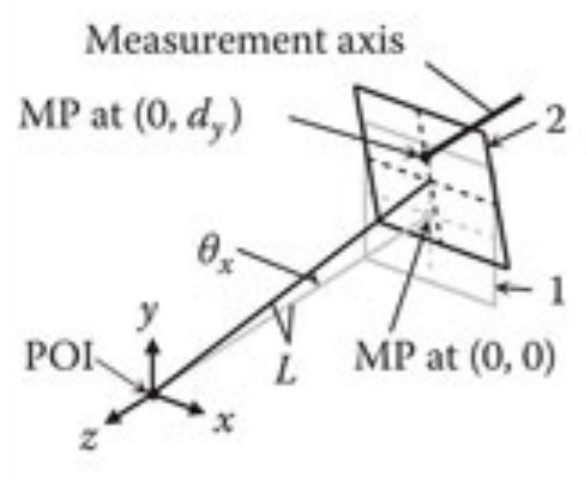
\includegraphics[width=3.5cm]{abbe-error}
		\caption{scheme used to understand the equation of the Abbe's error.} 
	\end{SCfigure}

	In order to eliminate the Abbe's error we can compensate by adding two more sensor (to determine $\theta_x,\theta_y$) that can determine the error $\abbe$. The same goal can be performed by analysing a sample problem: known it's value $L_m$, the computed measures is
	\[ L = L_m - d_y\tan\theta_x - d_x\tan\theta_y \]
	By evaluating this expression in two points (considering that an error, like $d_x\tan\theta_y$, can be consider negligible in respect to the other) by measuring an object more internal and external, we have a mathematical system that can be used in order to determine the unknown value $\theta_x$ and $L$. This method, in order to be successful, must consider that the angles $\theta_x$ and the length $L$ of the measure are invariant while changing the position of the sample.
	
	A smarter way to avoid the Abbe's error is just by doing a design choice minimizing the offset, so by making the line of motion collinear with the line of measurement.
	
	\paragraph{Cosine and sine error} The \de{cosine} error happens every time the measurement line is not parallel to the line of action. Considering the example of the measure of a length with a rule (as in figure \ref{fig:ps:cosineerror}) we can see that the measured length $L_m$ is different from the \textit{real} length $L$ of the object that we want to study, and in particular we can\ evaluate the difference in order to define the cosine error $\varepsilon_{\cos}$:
	\begin{equation}
		L = L_m \cos\alpha \qquad \Rightarrow \quad \varepsilon_{\cos} = L_m - L = L_m \big(1-\cos\alpha\big)
	\end{equation}
	
	\begin{SCfigure}[1.3][bht]
		\centering
		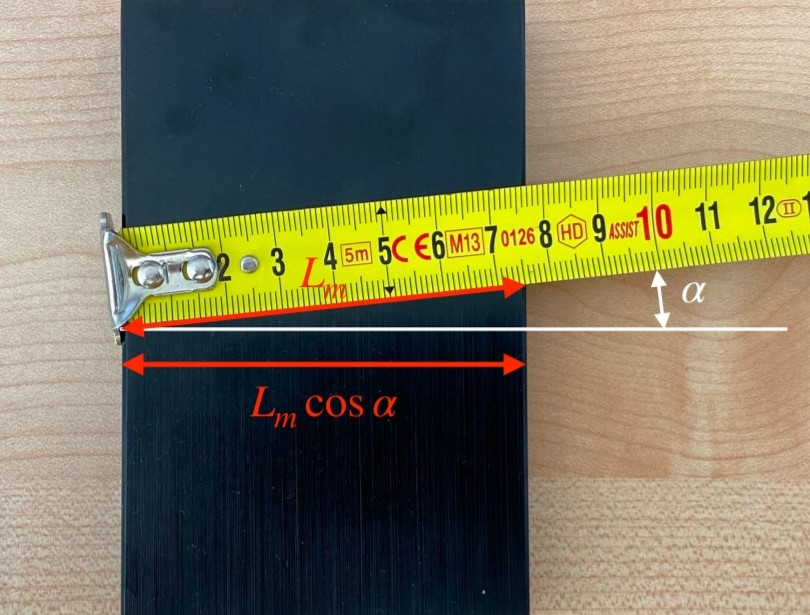
\includegraphics[width=5cm]{cosine-error}
		\caption{cosine error on a length measure.}  \label{fig:ps:cosineerror}
	\end{SCfigure}
	Extending the cosine error to a spatial environment we can compute  the error considering two angle $\alpha_x$ and $\alpha_y$ that can lead to an error:
	\begin{equation}
		\varepsilon_{\cos} = L_m\big(1-\cos\alpha_x\cos\alpha_y\big)
	\end{equation}
	\vspace{3mm}
	
	The \de{sine} error typically occurs when a physical contact is necessary for the measurement, like while dealing with the jaws of the calliper. By referring to figure \ref{fig:ps:sineerror} we can see that the error $\varepsilon_{\sin}$ is different in base of the geometry of the contact; considering as an example a flat-on-flat contact we can evaluate the error as
	\begin{equation}
		\varepsilon_{\sin} = \frac {w_z}2\sin\alpha_x + \frac{w_x}{2}\sin \alpha_z
	\end{equation}
	while considering instead a point contact the error reduces to the expression
	\begin{equation}
		\varepsilon_{\sin} = \frac {w_z}2\big(1-\cos\alpha_x\big) + \frac{w_x}{2}\big(1-\cos\alpha_z\big) = \frac{w_z}{2}\big(2-\cos\alpha_x-\cos\alpha_z\big)
	\end{equation}	
	
	
	\begin{SCfigure}[1.3][bht]
		\centering
		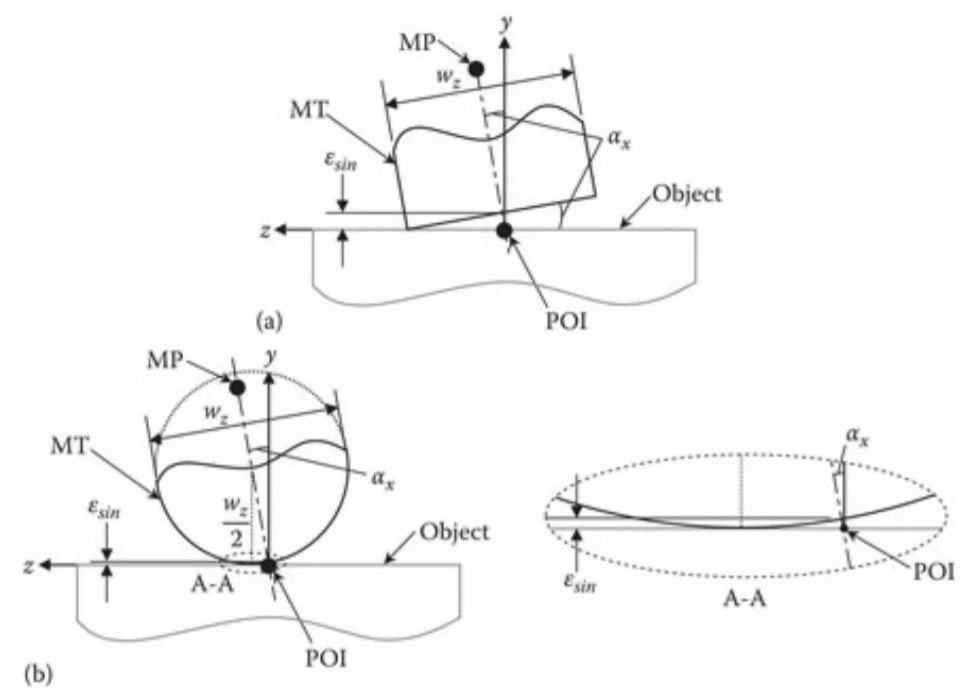
\includegraphics[width=5cm]{sine-error}
		\caption{sine error on a surface measure considering a flat-on-flat contact $(a)$ or a point contact $(b)$.}  \label{fig:ps:sineerror}
	\end{SCfigure}

	\paragraph{Alignment errors} In general Abbe's, cosine and sine errors are not mutually exclusive, so they can occur at the same time (Abbe's related to the offset, cosine due to a scale line not parallel to the  line of motion and the sine related to the angle between the moving jaw and the object).
	
	While designing measurement system it's important to determine all the specification that are useful to calculate the error factors that should be less then a decided value; this gives a suggestion on how to chose tolerances of the products.
	
	\begin{figure}[bht]
		\centering
		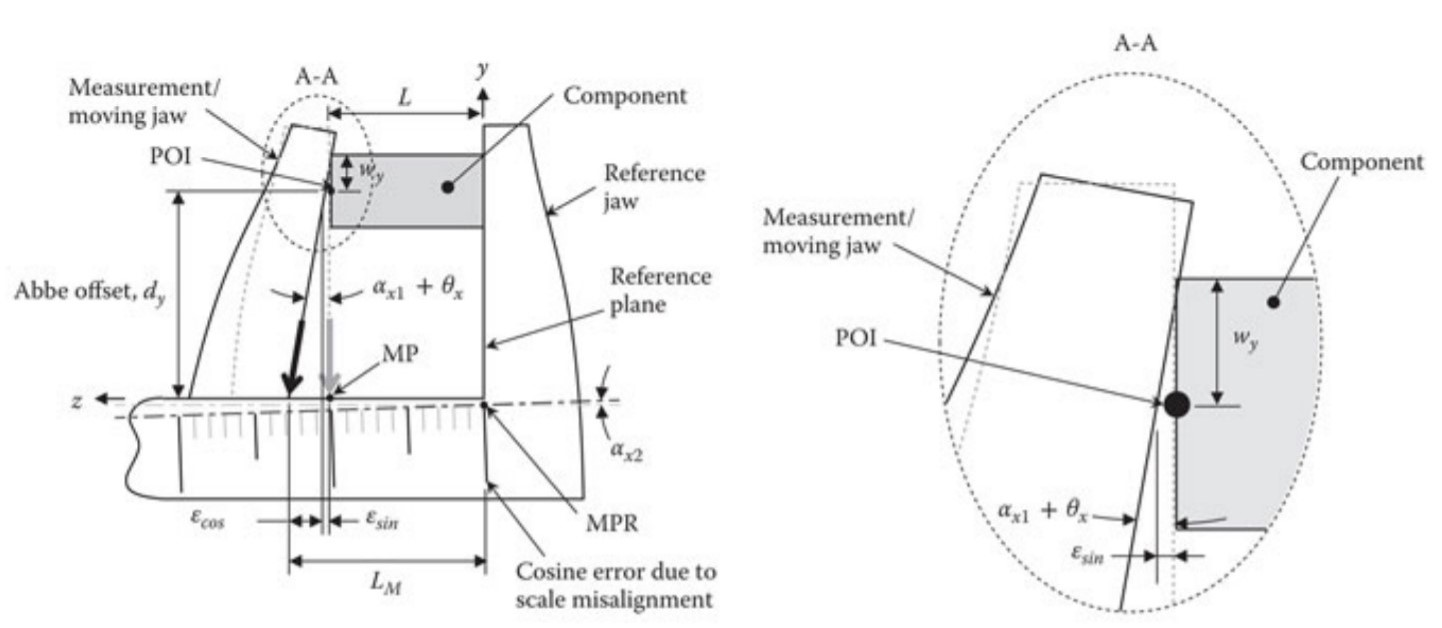
\includegraphics[width=10cm]{comb-errors}
		\caption{example of the combination of Abbe's, cosine and sine errors in a calliper.}
	\end{figure}
	
\section{Kinematics}
	
	In order to have a repeatable positioning it's important to minimize the internal stress by pursuing an isostatic design. When designing a system the kinematic analysis provides an understanding between the functional relationship between parts of mechanism, on how these parts are interconnected and how they move relative to each other.
	
	For example an unilateral constraint is represented by an inequality such $f(x,y,z) \geq 0$: in this step we usually consider bodies as \textbf{rigid}, so by considering part that are stiff enough in order to consider their deformation negligible in respect to the typical range of motion of the system. In precise machine it's important to consider all contact as rigid. \\
	In kinematic design we can assume that each	point of contact between two rigid bodies corresponds to a mutual constraint. In general if $f_j$ is the number of degrees of freedom of a joint $j$ having $n_{p_j}$ lowest number of contact point, than it's true that
	\begin{equation}
	\begin{split}
		\textrm{planar kinematics:}& \qquad f_j = 3 - n_{p_j} \\
		\textrm{spatial kinematics:}& \qquad f_j = 6 - n_{p_j} \\
	\end{split}
	\end{equation}
	
	Considering the more complex scenario of two line (straight or arcuate) contact, this is kinematically equivalent to two point constraints applied to any two different points along the contact line. 
	
	\begin{SCfigure}[2][bht]
		\centering
		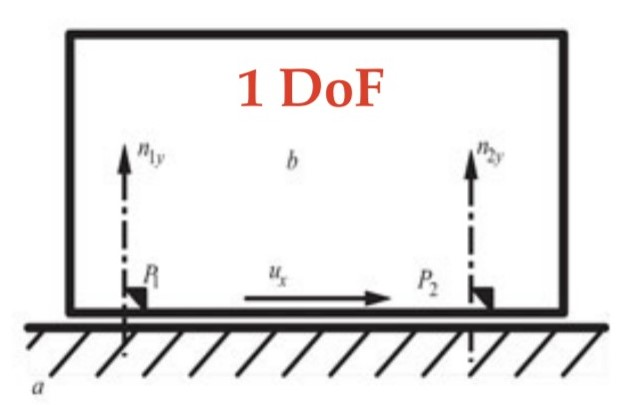
\includegraphics[width=3.5cm]{planar-contact}
		\caption{the contact of a body with straight line on a straight surface leads to two point constrains in order to have 1 degrees of freedom.}
	\end{SCfigure}
	
	\paragraph{Mobility of mechanisms} Considering now  a combination of $n$ rigid bodies constrained by $j$ joints can lead to a movable or immovable system. The net mobility of the mechanism is its number of degrees of freedom and can be calculated according to Tchebytchev as
	\begin{equation} \label{eq:ps:mobility}
		M = D\big(n-1-j\big) +\sum_i f_i = D\big(n-1\big) -\sum_j n_{p_j}
	\end{equation}
	where $D= 6$ for spatial mechanisms while $D= 3$ for planar kinematics. If $M>0$ then the mechanism is movable, for $M = 0$ the system is immovable while $M < 0$ it's over-constrained and so, in a real application, the structure will be subjected to unknown internal stresses that cannot be quantified (and so leading to imprecision).
	
	The Tchebytchev should be used with caution when dealing with systems that present singularities that can be determined by considering the position of the instantaneous centers of rotation of the bodies composing the system. Given a body $a$, it's instantaneous center of rotation in respect to the body $b$ is written as $P_{ab}$ and depends on the local configuration of the system. Every time that the center $P_{ij}$ goes to infinity, than the related configuration is singular and the Tchebytchev mobility calculation isn't correct.
	
	\paragraph{Over and under-constrained mechanisms} Under od over-constrained mechanisms can have unexpected side-effects that are often resulting in a lack of repeatability (unknown deformation of the system or unknown motion of some elements). As a consequence in precision engineering it is relevant to rely on kinematic design (which means exact constraint design) in order to have an isostatic system.
	
	\begin{figure}[bht]
		\centering
		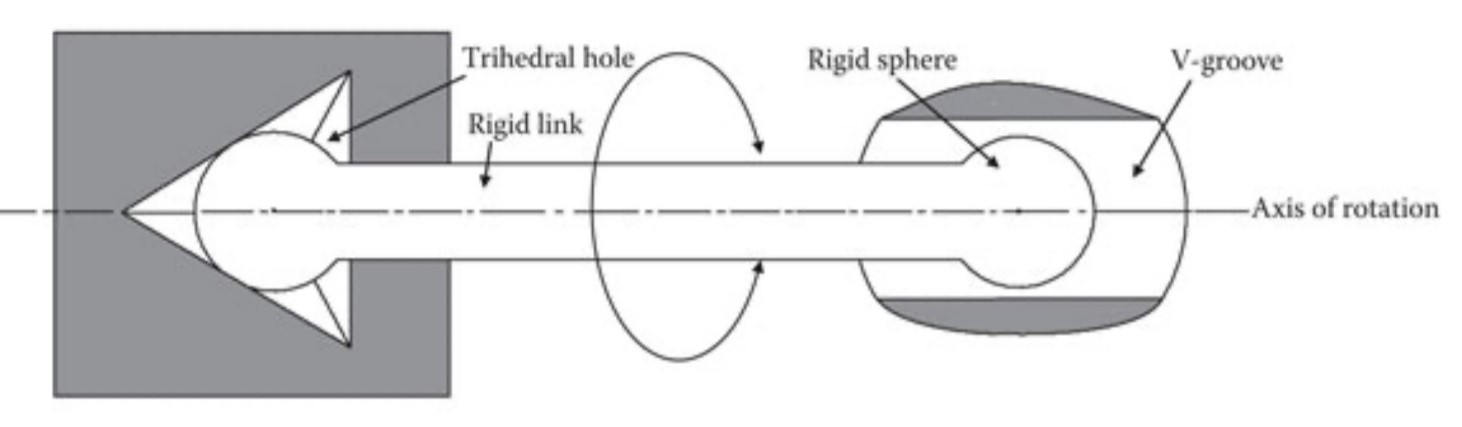
\includegraphics[width=7cm]{contactpointexample}
		\caption{example of a kinematic design of a rotary shaft.}
		\label{fig:ps:contactpointexample}
	\end{figure}

	Considering the example in figure \ref{fig:ps:contactpointexample} we can see that the tetrahedral groove determines 3 contact point, while the V groove add other 2, by determining a 1 degree of freedom of the shaft that's so free to rotate on it's axes. By replacing the V groove with another tetrahedral we have a $M=0$ and in order to have a mechanism that rotate we have to ensure that the shaft length is equal to the hole distance. An implementation of the previous kinematic design can be made with swivel ball (related to the V groove) and roller (tetrahedral) bearing as in figure \ref{fig:ps:contactsolution}.
	
	\begin{SCfigure}[2][bht]
		\centering
		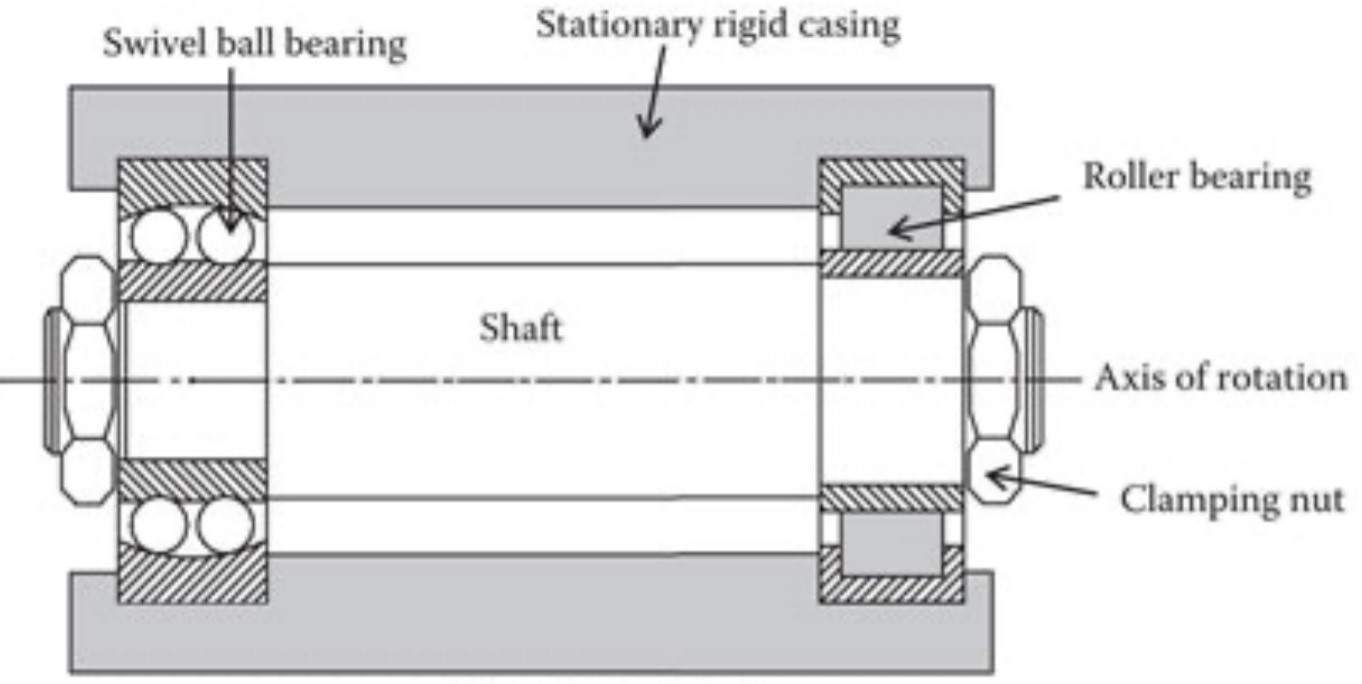
\includegraphics[width=6cm]{contactpointexample-sol}
		\caption{practical solution of the kinematic design of a rotary shaft drawn in figure \ref{fig:ps:contactpointexample}.}
		\label{fig:ps:contactsolution}
	\end{SCfigure}
	
	In general any deviation from purely kinematic design requires tighter tolerances and more stable materials that leads to increasing costs. In purely kinematic design it's required to use the minimum number of contact points that, as trade-off, increases the internal stress (and so decreasing the load capacity).
	
	\paragraph{Pseudo-kinematic design} To increase the load capacity we can use the so called \de{pseudo-kinematic design} by increasing the contact area while still providing constrains that are similar that are kinematic equivalent.
	
	\paragraph{Elastic averaging} Another approach that can be used to reduce the effects of machining inaccuracy is to use a large number of compliant coupling in order to spread the errors on a large area.	An example of this technique can be seen in figure \ref{fig:ps:elasticaveraging}.
	
	\begin{figure}[bht]
		\centering
		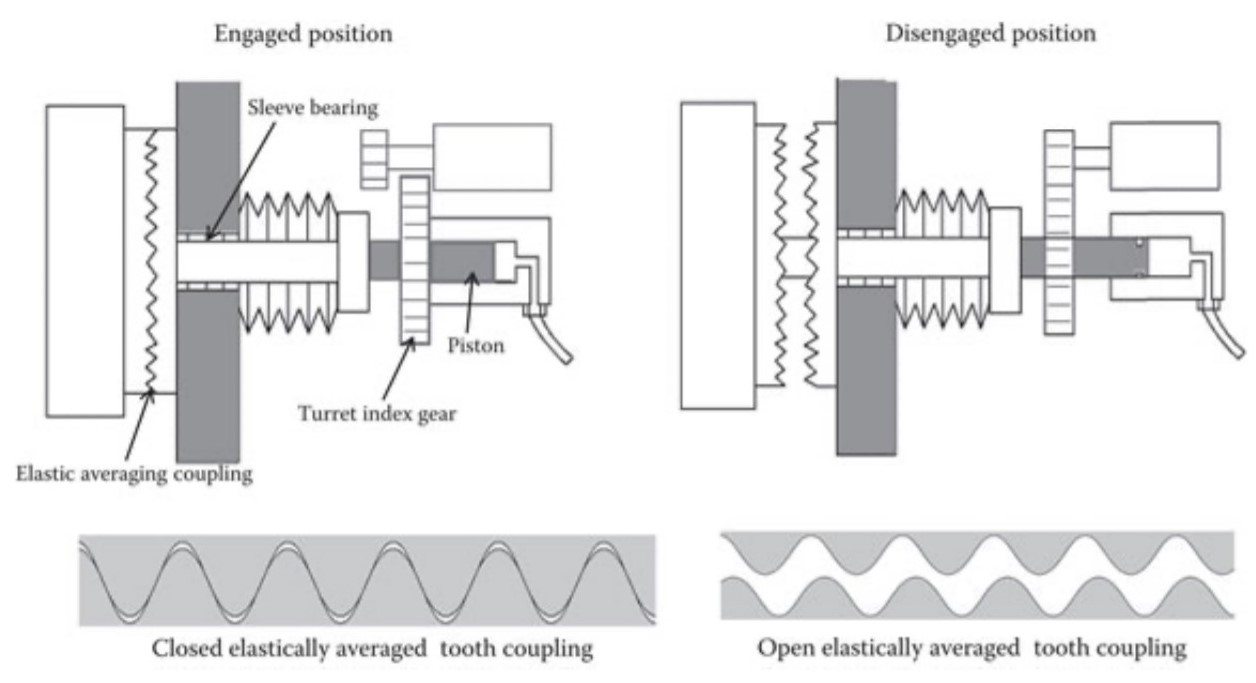
\includegraphics[width=9cm]{elasticavereging}
		\caption{example of a system that uses elastic averaging in order to better create a kinematic connection between two components.}
		\label{fig:ps:elasticaveraging}
	\end{figure}
	
	\subsection{Kinematic couplings}
		When designing a precision assembly we often need to precisely locate two subsystems respect to each other; sometimes we also want to isolate effects of strains acting on the frame element from a carried subsystem. In all this cases the coupling must be kinematic (by so determining a mobility $M=0$) in order to decouple the carried subsystem from effects of the carrier (like mechanical and thermals strains, manufacturing errors...).
		
		One of the most common type of kinematic coupling is the \textbf{Kelvin clamp} as in figure \ref{fig:ps:kelvinclamp}. In general good coupling design shall avoid overconstrained geometries (as example a pillar that have to support a high load, we don't use a pure flat surface but only a perimeter part of the cross section in order to minimize the surface in contact).
		
		\begin{SCfigure}[2][bht]
			\centering
			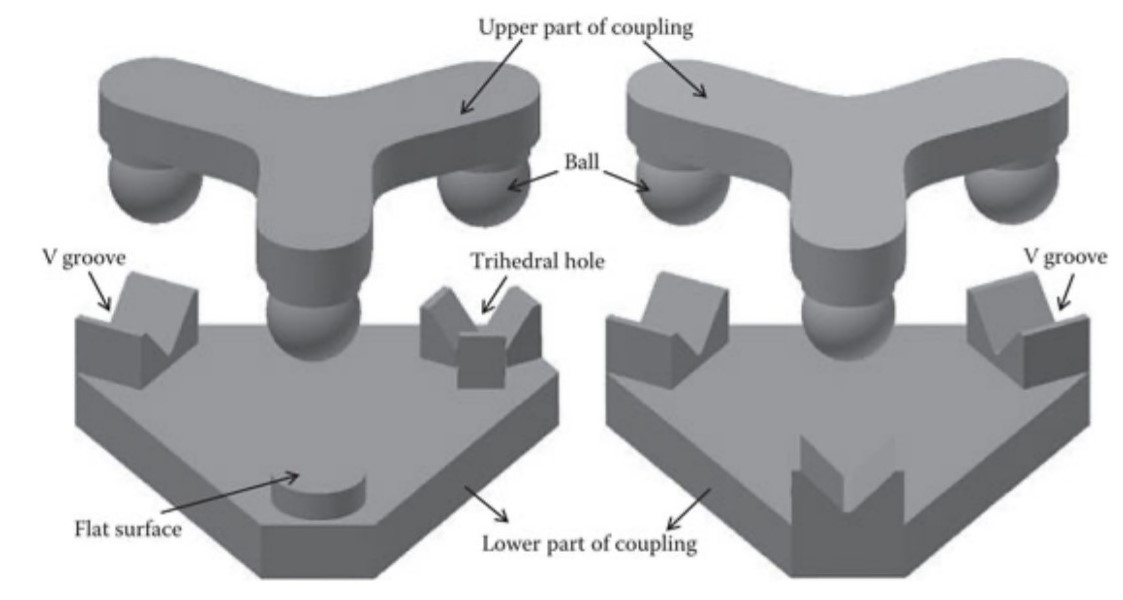
\includegraphics[width=6.5cm]{kelvinclamp}
			\caption{Kelvin clamp of type I (on the left) and type II (right).} 
			\label{fig:ps:kelvinclamp}
		\end{SCfigure}
		
	\subsection{Hertzian contacts} 
		In order to describe the elastic interaction between contact point we can use the theory of the \de{Hertzian contacts} that allows to compute the pressure $p(r)$ and contact stiffness $K_n$ of a sphere on a sphere (or on a plane considering $R_2$ that tends to infinity). In particular the pressure $p$ on the surface, the displacement $\delta$ the contact stiffness $K_n$ can be calculated, depending on the applied force $F_n$, as
		\begin{equation}
			p(r) = p_0 \sqrt{1- \frac{r^2}{a^2}} \qquad \delta = \frac{a^2}{R} = \sqrt[3]{ \frac{9F_n^2}{16\overline E^2 R} } \qquad K_n = \frac{dF_n}{d\delta} = 2\overline E \sqrt{\delta R}
		\end{equation}
		when the parameters can be computed as
		\[ p_0 = \sqrt[3]{\frac{6 F_n E^2}{\pi^3 R^2}} \qquad a = \sqrt[3]{\frac{3F_n R}{4\overline E}}  \]
		In order to compute the average $\overline E$ of the Young modules and the equivalent contact radius $R$ the following expression must be considered:
		\[\frac 1 {\overline E} = \frac{1-\nu_1^2}{E_1} + \frac{1-\nu_2^2}{E_2} \qquad \frac 1 R = \frac 1 {R_1} + \frac 1 {R_2}\]
		\begin{SCfigure}[3][bht]
			\centering
			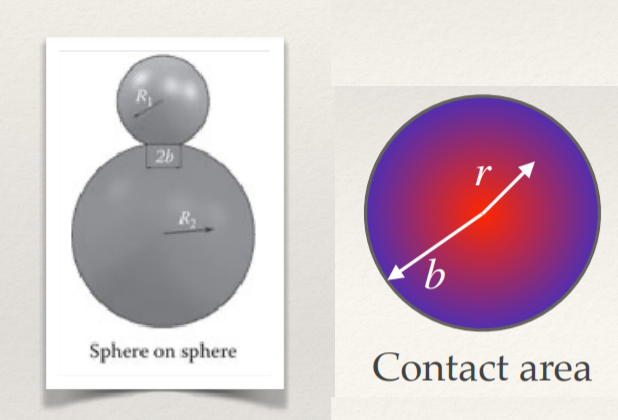
\includegraphics[width=5cm]{hertian-point}
			\caption{scheme to refer when considering the hertzian contact of a sphere on a sphere. On the left the macro picture of the contact with the main dimensions and on the left the heap map of the pressure distribution on the contact surface.}
		\end{SCfigure}
		
		Considering instead the contact of a cylinder on a cylinder the surface pressure $p$ and it's displacement $\delta$ depends from the deviation $x$ on the ideal contact line and are equals to
		\begin{equation}
			p(x) = p_0 \sqrt{1- \frac{r^2}{b^2}} \qquad \delta = \frac{F_n}{\pi \overline E L} \left[ 1 + \ln \left(\frac{\pi L^3\overline E}{PR}\right) \right]
		\end{equation}
		where
		\[ p_0 = \frac{2F_n}{\pi b L } = \sqrt{\frac{F_b\overline E}{\pi RL}} \qquad b = \sqrt{\frac{4F_nR}{\pi \overline E L}}  \]
		
		\begin{SCfigure}[2][bht]
			\centering
			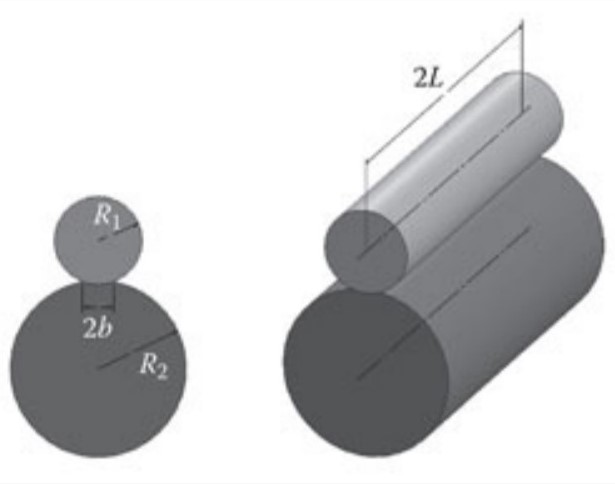
\includegraphics[width=4cm]{hertian-cyl}
			\caption{scheme to refer while considering the hertzian contact of two cylinders.}
		\end{SCfigure}
	
		\paragraph{Dowel pins} A common need is to precisely mount a plate onto a base and this operation is often performed by the \textbf{dowel pins}: each pin locks one degree of freedom on the plane, so 3 pins can be used to kinematic constrain a plate in a planar kinematic. In reality this pins are unilateral constrains and so a 4-th locking point is needed.
		
		\textbf{DISCORSO SUL CALCOLO DEI MOMENTI ROTAZIONE PER CAPIRE SE I PIN SONO SUFFICIENTI, MAGARI RIVEDERE LEZIONE}
	

\section{Flexure hinges}
	\de{Flexure hinges} are made as a substitute to the conventional rotational joint by using an elastic deformation of a single element (so with no movable part) that allows to have a more repeatable motion of the mechanism.
	
	Relative motion between two members of a mechanism can in fact be implemented by sliding/rolling (that introduces a certain degree of backlash and so uncertainty due to physical phenomena such friction, hysteresis, roughness...) or by using an elastic deformation (that's more reliable in terms of accuracy and so repeatability); the only drawback of this kind of hinges is that they are repeatable nut only in a limited extent (in order to maintain the elastic property of the material). Usually this kind of connection is cheaper. 
	
	A \de{flexure} (or \textbf{flexure hinge}) is a localized volume in a rigid body that presents much higher flexibility (or lower stiffness in other words) typically thanks to a significant reduction in the cross section. In a lumped model, flexure hinges can be considered as springs.
	
	\paragraph{Leaf spring} The simplest type of rotary flexure hinge is the \textbf{leaf spring} that's behaves as a cantilever beam like in figure \ref{fig:ps:cantbeam}.
	
	\begin{SCfigure}[1][bht]
		\centering 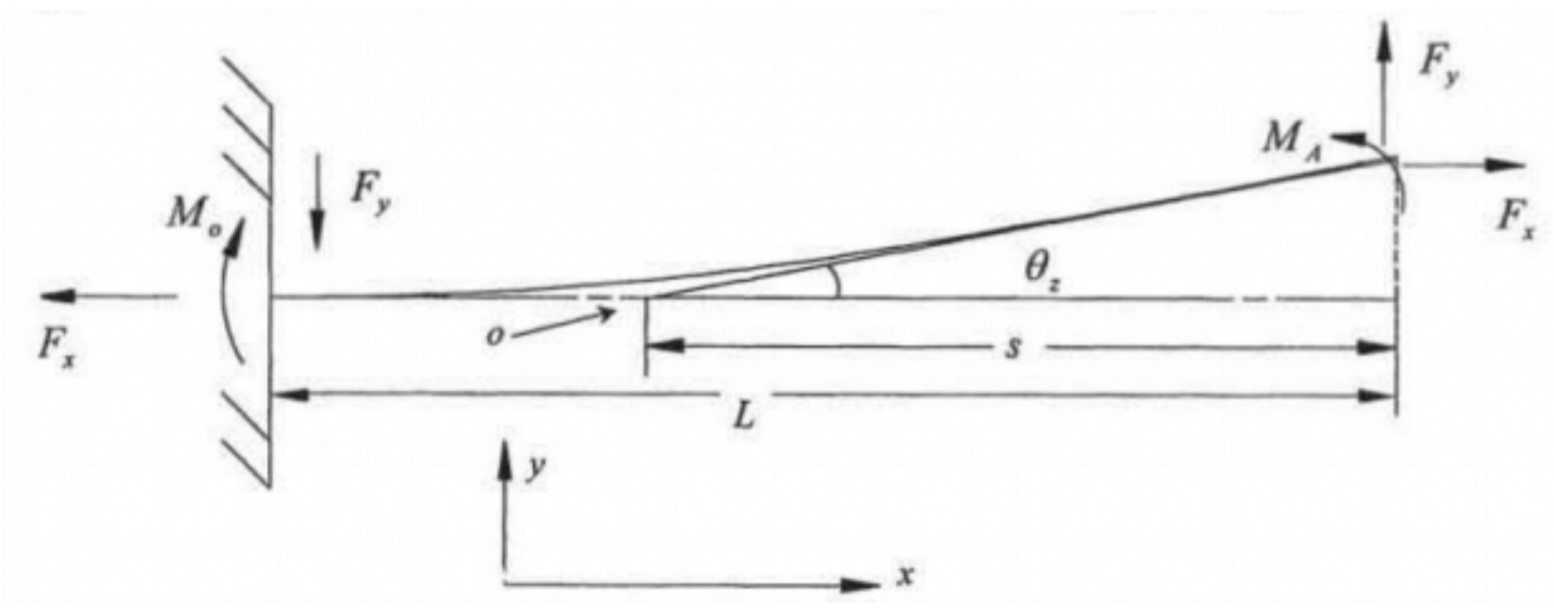
\includegraphics[width=8cm]{cantileverbeam}
		\caption{leaf spring model of the flexure hinge as a cantilever beam.}
		\label{fig:ps:cantbeam}
	\end{SCfigure}
	
	From  thin beam theory it's possible to compute the bending moment for a generic distance $x$ from the constraint as
	\[ M(x) = F_y (L-x) = EI \frac{d^2y}{dx^2} \]
	By integration of this relation we can compute the deflection $y(x)$ of the beam and it's slope $\theta(x) = dy/dx$:
	\begin{equation}
	\begin{aligned}
		EI \frac{dy}{dx} & = F_y \left( FX - \frac{x^2}{2} \right) + c_1 \qquad & \Rightarrow \quad \theta(x) &= \frac{F_y}{EI} \left(Lx - \frac{x^2}{2}\right) \\
		EI y & = F_y \left(L\frac{x^2}{2} - \frac{x^3}{6}\right) +c_1 x + c_2\qquad & \Rightarrow \quad y(x) &= \frac{F_y}{EI} \left(L\frac{x^2}{2} - \frac{x^3}{6}\right) 		
	\end{aligned}
	\end{equation}

	In the hypothesis of small displacements the slope $\theta_z$ of the beam is equal to the angle measured at the tip and also the vertical displacement $\delta_y$ can be computed as
	\begin{equation}
		\theta_z = \theta(L) = \frac{F_y L^2}{2EI} \qquad \delta_y = y(L) = \frac{F_yL^3}{3EI}
	\end{equation}
	
	This expression also allows to compute the angular and linear stiffness by considering different set of displacement/actions:
	\begin{equation}
		k_{\theta_zF_y} = \frac{F_y}{\theta_z} = \frac{2EI}{L^2} \qquad k_{\theta_zM_z} = \frac{M_z}{\theta_z} = \frac{2EI}{L} \qquad k_{\delta_y F_y} = \frac{F_y}{\delta_y} = \frac{3EI}{L^3}
	\end{equation}
	
	Given the maximum allowable deflection slope $\theta_{max}$, we can calculate the maximum thickness $t$ (in $y$ direction in respect to figure \ref{fig:ps:cantbeam}) of the hinge in order not to yield the material by satysfying the relation
	\begin{equation}
		\frac{Et}{2L} \theta_{max} \leq \sigma_y \qquad \Rightarrow \quad t \leq \frac{2L}{E\theta_{max}} \sigma_y
	\end{equation}
	This also gives the maximum stiffness as 
	\[ k_{\theta_zM_z,max} = \frac{2EI_{max}}{L} = \frac{2Ebt^3_{max}}{12L} = \frac{4bL^2}{3E^2}\left(\frac{\sigma_y}{\theta_{max}}\right)^3 \]
	
	By using the cantilever as a hinge, we need to know the location of the pivot point (defined by the length $s$ as in figure \ref{fig:ps:cantbeam}); although it depends on the amount of deflection, for small displacements even the displacement of the pivot point is small. So we can assume it has its initial position at the intersection between the two tangents at the free and at the at the constrained edge of the beam by giving the length
	\[ s = \frac{\delta_y}{\tan\theta_z} \simeq \frac 2 3 L \]
	so in general we can consider the the pivot point of a cantilever leaf spring is located at $1/3$ of it's length from the fixed end. \\
	In general this kind of hinge presents better response on traction than compression (where instability might occur). Multiple leaf springs can be combined to realize mechanisms, as a four-bar-linkage, obtained from a single block of metal machine by wire-EDM (\textit{elettro erorsione}).
	
	More complex equations can consider also the axial load $F_x$ and torque moment $M_z$, but for now we neglect
	\begin{note}
		More information can be found on the book \textit{Flexure Elements of Elastic Mechanisms} (Stuart T. Smith), chapter 4.1.
	\end{note}

	\subsection{Notch hinge}
		A \de{notch hinge} (figure \ref{fig:ps:notch-hinges}) is easier to manufacture (respect to the leaf spring) and it's composed by a beam with two notches of circular/elliptical/rectangular shape. The main parameter $\varepsilon$ allows to define how \textit{circular} ($\varepsilon = 1$) or \textit{rectangular} ($\varepsilon\rightarrow \infty$) the notch is and it's defined as
		\begin{equation}
			\varepsilon = \frac{a_x}{a_y} \qquad \beta = \frac{t}{2a_x}
		\end{equation}
	
		\begin{figure}[bht]
			\centering
			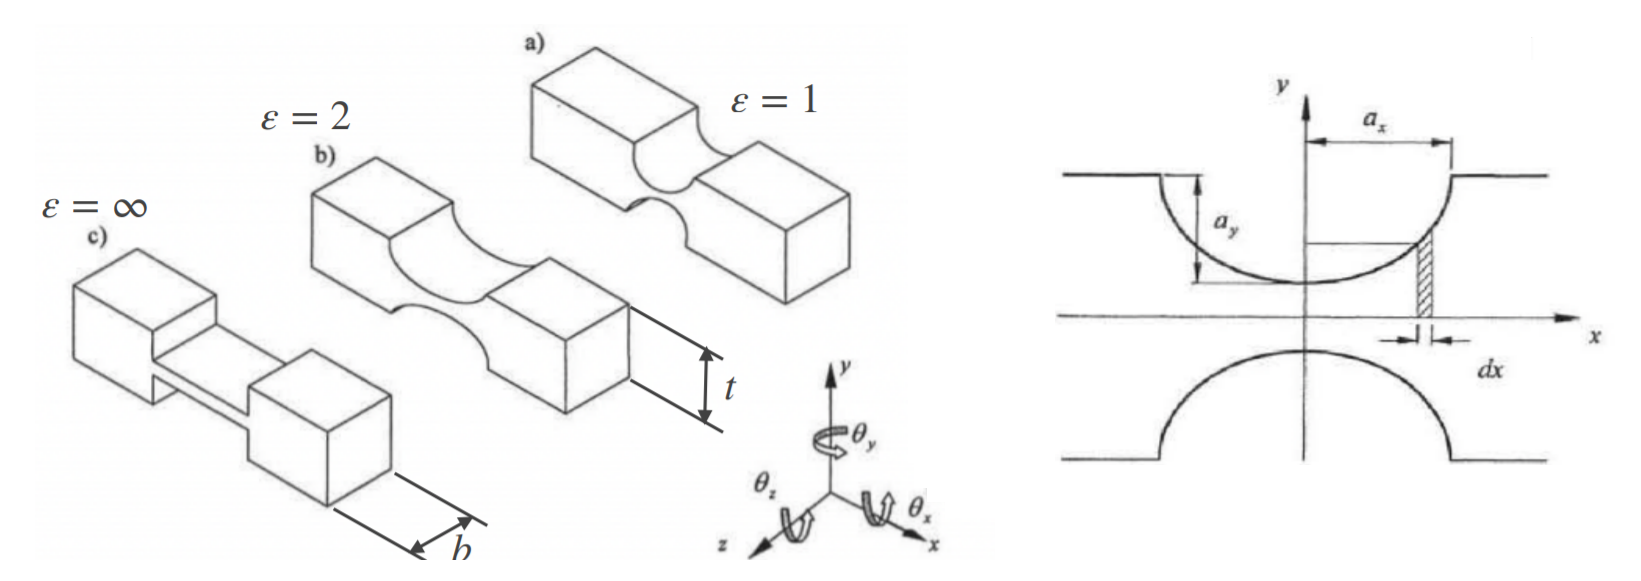
\includegraphics[width=10cm]{noth-hinges}
			\caption{examples of notch hinges depending on the parameters $\varepsilon$ and technical drawings used to compute $\varepsilon,\beta$.}
			\label{fig:ps:notch-hinges}
		\end{figure}
	
		Related to this kind og hinges we can define the moment stiffness (that depends on a \textit{complex} function $f$ of the parameter $\beta$) with a particular approximation for small values of $\beta$:
		\[ k_{\theta_zM_z} = \frac{2Rb a_x^2}{3f(\beta)} \approx \frac{2Eba_x^2}{3} \frac{\sqrt[2]{(2\beta)^5}}{3\pi} = \frac{2Eb \sqrt {t^5}}{9\pi \sqrt{a_x}} \]
		The true  stress $\sigma$ can be determined as function of the applied moment $M_z$ ot the rotation $\theta_z$:
		\[ \sigma = \sqrt[20]{(1+\beta)^9} \frac{6M_z}{t^2b} = \frac{4 E a_x^2 }{f(\beta)t^2}\sqrt[20]{(1+\beta)^9} \theta_z = \frac{ E \sqrt[20]{(1+\beta)^9}}{\beta^2 f(\beta)} \theta_z \]
		
		By considering that $\sigma$ should always be less than the yielding strength (to avoid yielding) we can compute the maximum thickness $t_{max}$ of the notch hinge to avoid this phenomena:
		\[ t_{max} = \sqrt{ \frac{4Ea_x^2}{f(\beta)} \sqrt[20]{(1+\beta)^9} \frac{\theta_z}{\sigma_{ys}} } \]
		\textbf{MANCA LA FORMULA APPROSSIMATA CHE è DA CHIEDERE AL PROFESSORE}
		
		With this consideration we can also define the maximum angular stiffness as
		\[ k_{\theta_z M_z,max} = \frac{\pi^4 b a_x^2}{19 \sqrt[4]{1+\beta}E^4 } \left( \frac{\sigma_{ys}}{\theta_z} \right) \]
		
		
		\vspace{3mm}
		
		This kind of hinges are used only when low angle deflection are required ($10-15^\circ$), while when larger deflections are used it might be better to use \textbf{cross street pivot}  or a \textbf{cartwheel hinge} (figure \ref{fig:ps:cartwheelhinges}); this solutions are preferred with respect to the leaf spring due to the fact that the pivot point/hinge axes is fixed and doesn't move depending on the displacement.
		
		\begin{SCfigure}[1][bht]
			\centering
			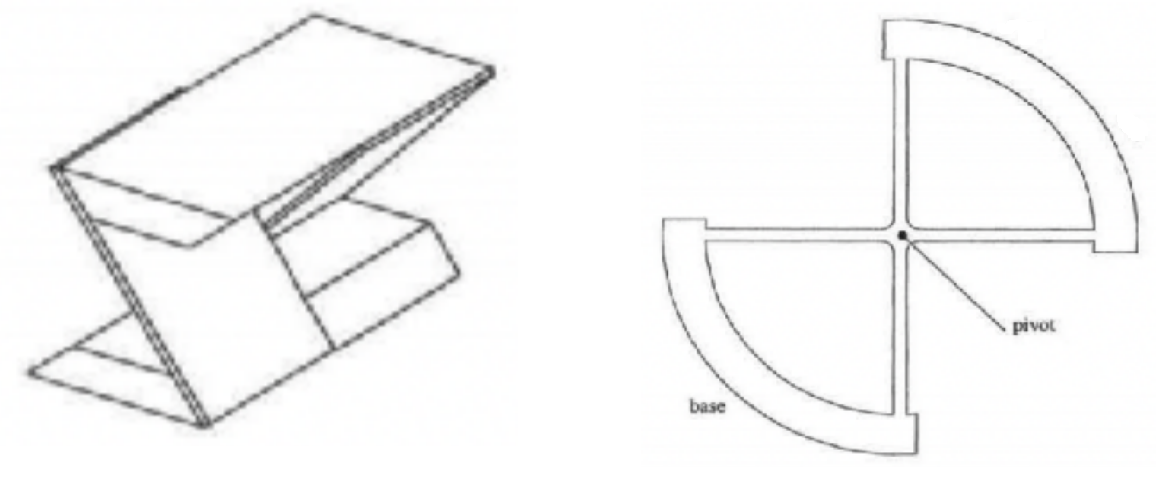
\includegraphics[width=6cm]{cartwheel-hinge}
			\caption{cross street pivot (on the left) and cartwheel (right) hinges.}
			\label{fig:ps:cartwheelhinges}
		\end{SCfigure}
		
		An other way to create a cross strip pivot is by installing (with a rotation of $90^\circ$ relative angle) 2 orthogonal drilled notch hinges as shown in figure \ref{fig:ps:crossstrip}.
		
		\begin{SCfigure}[1][bht]
			\centering
			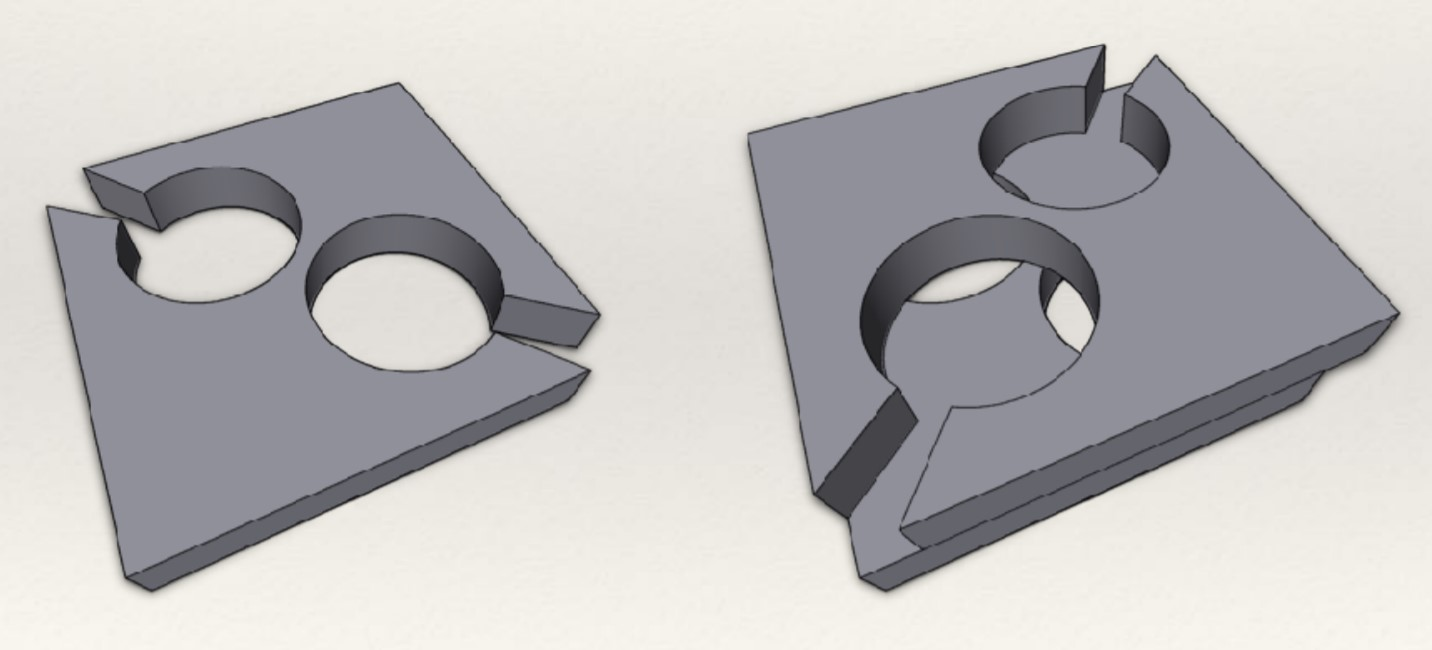
\includegraphics[width=6cm]{cross-strip}
			\caption{example of a cross strip pivots realised with 2 orthogonal drilled notch hinges.} \label{fig:ps:crossstrip}
		\end{SCfigure}
		
		
		To create high precision system is recommended the use of metals (instead of plastic) in order to reduce the effect of the hysteresis on the flexure hinges.
	
	
	\subsection{Rectilinear motion mechanism with flexure hinges}
		\paragraph{Flexure system} A \de{flexure system} is a mechanism implemented with rigid bodies connected by flexure hinges; typically it's a monolithic structure (so made by one whole piece). This kind of systems limits as much as possible the number of components hence improving precision (in fact there are no hysteresis, friction but also the interaction between different materials). \\
		If we want to deal with multiple materials we have to ensure kinematic coupling in order to avoid undesired force transmission due to thermal changes on the components.
		
		\paragraph{Simple linear spring mechanism} A linear spring mechanism can be implemented as a quadrilateral with parallel links.
		
		\begin{SCfigure}[2][bht]
			\centering
			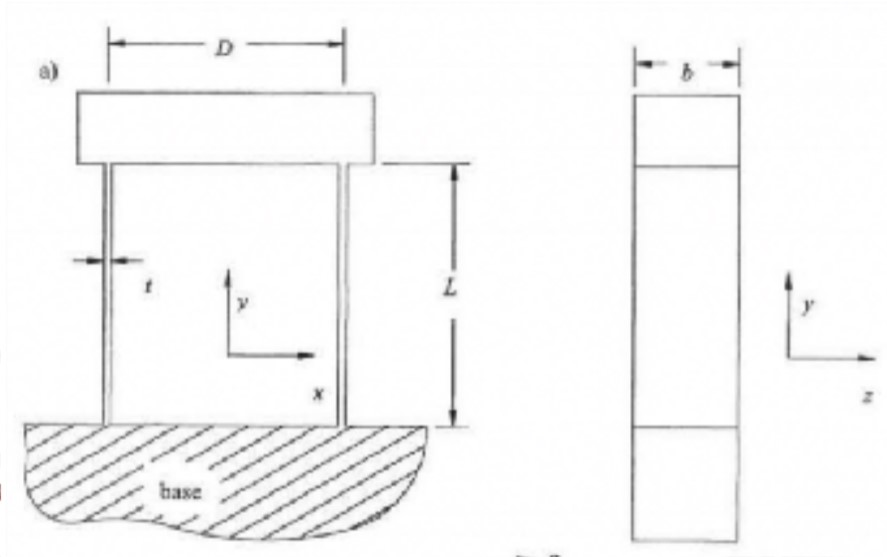
\includegraphics[width=6.5cm]{rect-spring}
			\caption{implementation of a rectilinear motion with leaf spring flexures.}
			\label{fig:ps:rect:spring}
		\end{SCfigure}
	
		When using leaf spring flexures, as shown in figure \ref{fig:ps:rect:spring}, the stiffness along the $x$ axis can be computed considering the 4 hinges as
		\[ k_{\delta_xF_x} = \frac{24EI_{zz}}{L^3} = 2 Eb \left( \frac tL\right)^3 \]
		Doing an impedances analyses it also possible to compute the free natural frequency of the system that's equal to
		\[ f_{n_x} = \frac{\omega_{n_x}}{2\pi} = \frac{1}{2\pi} \sqrt{\frac{k_{\delta_xF_x}}{M + \frac{26}{35}m}} = \frac 1 {2\pi} \sqrt{\frac{24 EI_{zz}}{L^3\left( M + \frac{26}{35}m \right)} }  \]
		where $m$ is the mass of the suspended bar while $M$ is the mass of the leaf spring bar.
		
		The same mechanism of mechanism can be also realised considering the usage of notch hinges (instead of the leaf spring) as in figure \ref{fig:ps:rect:notch}.
		
		\begin{SCfigure}[2][bht]
			\centering
			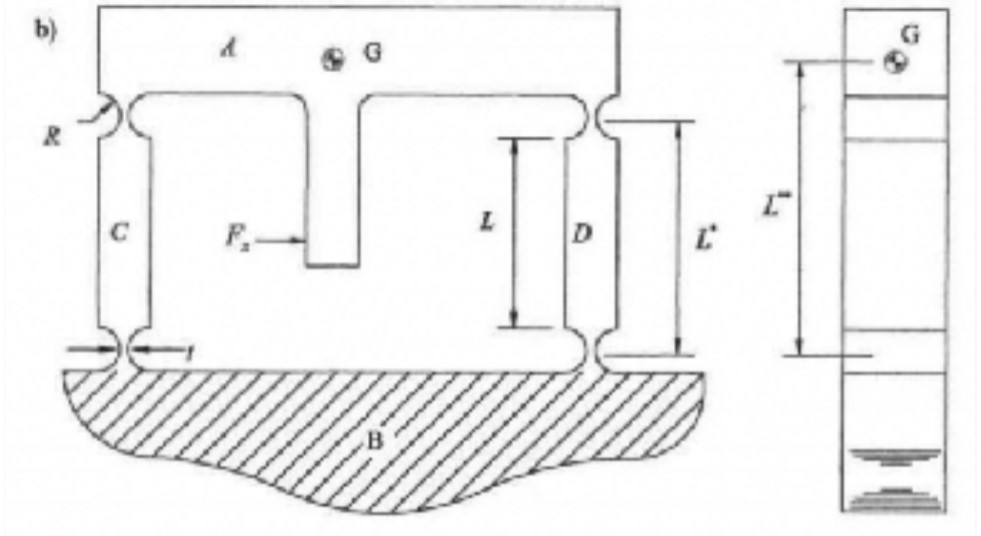
\includegraphics[width=6.5cm]{rect-notch}
			\caption{implementation of a rectilinear motion with notch hinges.}
			\label{fig:ps:rect:notch}
		\end{SCfigure}
	
		This system behaves differently and determines a different angular stiffness and natural frequency response (that's usually higher than the leaf spring implementation):
		\begin{align*}
			k_{\delta_xD_x} & = \frac{F_x}{\delta_x} = \frac{4 k_{\theta_zM_z}}{L^{*2}} = \frac{8 E b \sqrt{t^5}}{9\pi \sqrt R L^{*2}} \\
			\omega^2_{n_x} & = \sqrt{\frac{4k_{\theta_zM_z}}{M_AL^{*2} + 2 M_CL^2\left( \frac 1 3 + \frac R L + 4\frac{R^2}{L^2} \right)  }}
		\end{align*}
		
		This kind of mechanism, for slow deviation of the tip, can be approximated as a linear motion; sometimes for particular application the mechanism should realize a circular motion, and for small angles that can be defined considering the instantaneous center of rotation of the four bar linkage as the example in figure \ref{fig:ps:circmotion}.
		
		\begin{SCfigure}[2][bht]
			\centering
			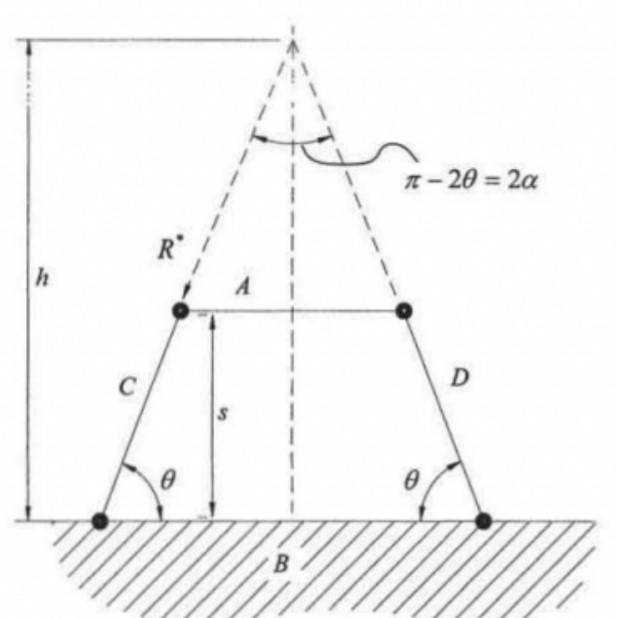
\includegraphics[width=5cm]{circular-motion}
			\caption{four bar linkage realised with flexure elements that allows circular motion of the top bar (for small deviations).}
			\label{fig:ps:circmotion}
		\end{SCfigure}
		
		Considering that mechanism the points on the top bar $A$ are set to follow a circular motion in respect to the instantaneous center of rotation (this approximation holds for small deviation from the nominal position) and in particular given the length $l_i$ of the various bars we can compute the distance $h$ of the center of instantaneous rotation and the radius $R^*$ of the circular motion as
		\begin{align*}
			h & = \frac{l_B s}{l_B-l_A} \\
			R^* & = \frac{l_As}{\big(l_B-l_A\big) \cos\left(\frac \pi 2 -\theta\right) = \frac{l_Al_C}{l_B-l_A} }
		\end{align*}
	
		In general this kind of mechanisms are reliable only of the stiffness of the hinges is lumped, so it's very localized in order to consider linkages way much stiffer (rigid bodies) for most of the part.
		
		\paragraph{Compound rectilinear spring} If we have a strong specification on motion rectilinearity we can use a \textbf{compound rectilinear mechanism} to ensure this requirement.
		
		\begin{SCfigure}[2][bht]
			\centering
			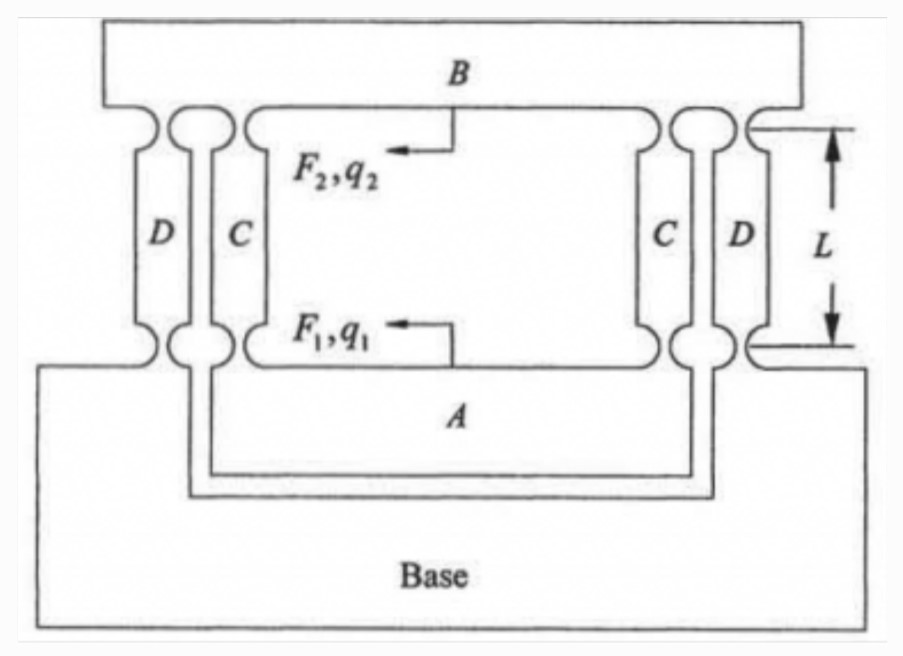
\includegraphics[width=5cm]{rect-comp-1}
			\caption{compound rectilinear spring used to increase the linearity of the motion on the plate $A$.}
			\label{fig:ps:rect:comp}
		\end{SCfigure}
		
		Considering the Tchebytchev equation \ref{eq:ps:mobility} (page \pageref{eq:ps:mobility}) we have that the mobility of the mechanism is equal to $2$ and so we have two coordinates (in this case $x_A,x_B$) we have more complex natural modes of the system but this allows to have a linear motion of the block $A$ in respect to the base (considering that all the hinges presents the same stiffness). Also this consideration holds considering quasi-static movement (so ignoring the inertia of the part composing the system).
		
		Joining this compounded rectilinear spring with a mirrored version (as in figure \ref{fig:ps:rect:mirrcomp}) we define a mechanism with one degree of mobility (according to Tchebytchev) even on non static conditions. This implementation also present built-in hard stops that prevents the yielding of the hinges while deflecting.
		
		\begin{SCfigure}[2][bht]
			\centering
			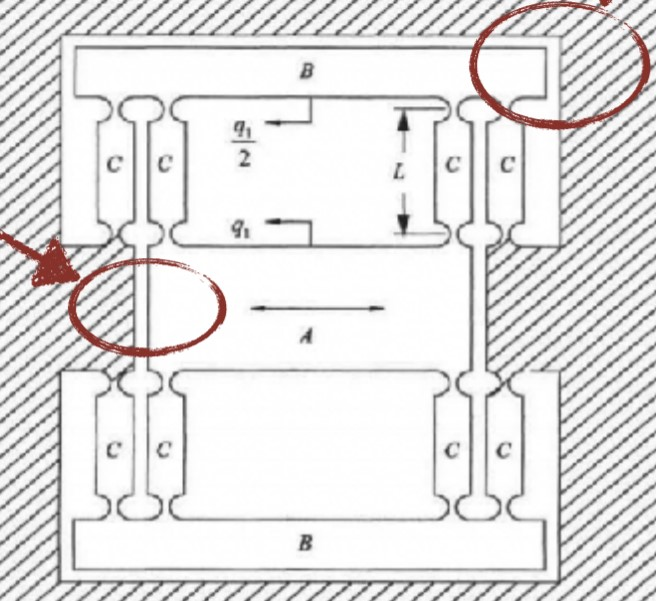
\includegraphics[width=5cm]{rect-comp-2}
			\caption{improved compound rectilinear spring from the version in figure \ref{fig:ps:rect:comp} with mobility $M=1$ obtained by joining the original piece with a mirrored copy. The red circles shown the hard stop of motion realized by the frame in order to avoid yielding.}
			\label{fig:ps:rect:mirrcomp}
		\end{SCfigure}
	
	\subsection{Flexure levers}
		While dealing with precision system another function that's needed is the the mechanical gain that can be obtained by a lever: in flexure system we refer to this functions as \de{flexure levers}. In particular when the gain is larger than 1, than the displacement is amplified (typically used on sensors), while when the gain is smaller than one allows to perform micro positioning (used on actuators). We have to consider that swapping input and output the gain inverses.
		
		This kind of mechanism can be realised with \textbf{rigid} levers or by using combination of \textbf{soft-sprint/stiff-spring} attenuation configurations (used for precise actuators), like the one in figure \ref{fig:ps:softstiff}.
		
		\begin{SCfigure}[1][bht]
			\centering
			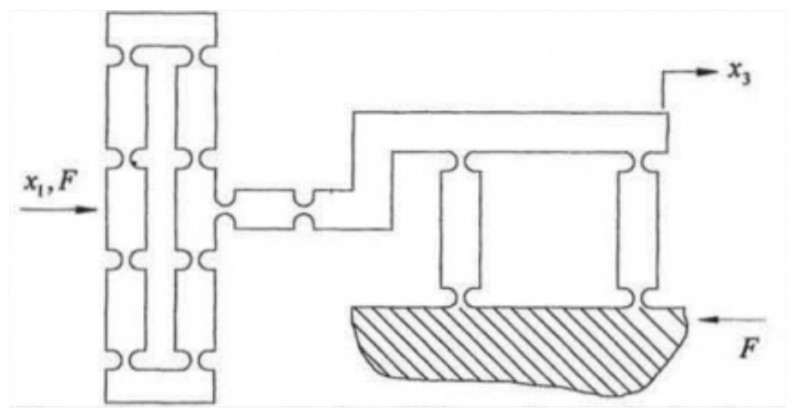
\includegraphics[width=6cm]{soft-stiff-lever}
			\caption{example of a soft-spring/stiff-spring attenuation flexure mechanism.}
			\label{fig:ps:softstiff}
		\end{SCfigure}
		
		When talking about a lever we define the \textbf{lever ratio} $n$ as
		\begin{equation}
			n = \frac{\textrm{output displacement}}{\textrm{input displacement}} = \frac{x_1}{x_2}
		\end{equation}
		Considering figure \ref{fig:ps:leverpoint} we can see that when the pivot point is between the input and the output we have $n = \frac ba$, while when the pivot is on the outside the ratio become $n = \frac{a+b}{a}$.
	
		\begin{figure}[bht]
			\centering 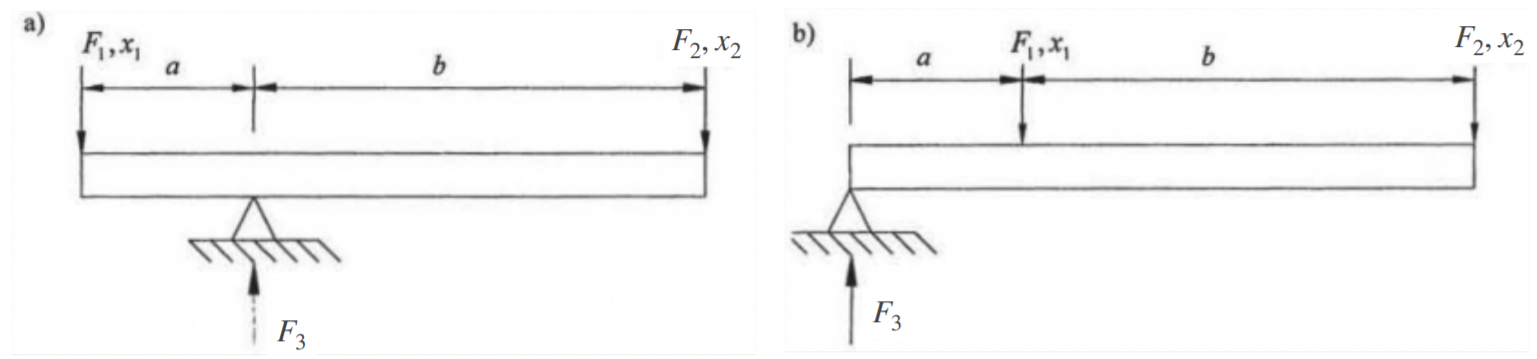
\includegraphics[width=12cm]{leverpoint}
			\caption{example of levers where the pivot point is between (on the left) or on the outside (right) respect to the pivot point.}
			\label{fig:ps:leverpoint}
		\end{figure}
	
		\paragraph{Two bar lever} Let's consider the case of a two bar lever (as in figure \ref{fig:ps:twovarlever}) for which, using the Tchebytchev formula (eq. \ref{eq:ps:mobility}), the system present one degree of freedom.
		
		\begin{SCfigure}[2][b]
			\centering
			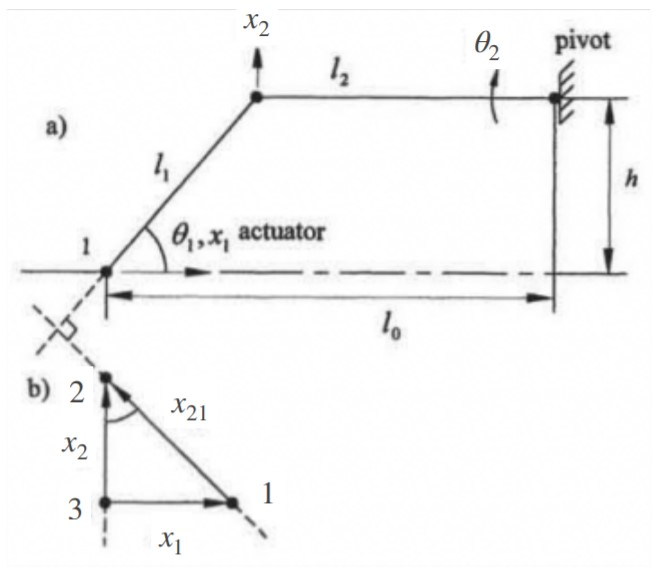
\includegraphics[width=5cm]{two-bar-lever}
			\caption{schematic representation (with main design parameters) of a two bar lever.} \label{fig:ps:twovarlever}
		\end{SCfigure}
		In this case the point $3$ is the pivot (with so a fixed position); considering the sketched length of the bar it's possible to compute the lever ratio considering that the input position is $x_1$; in particular noting that the displacements can be computed $x_1 = x_2\tan\theta$, then we can observe how the lever ratio depend on the cotangent of the angle $\theta_1$ between the two bars:
		\[ x_2 \tan \theta_1 = x_1 \qquad \Rightarrow \quad n = \cot\theta_1 = \frac{l_0-l_2}{h} = \frac{\sqrt{l_1^2-h^2}}{h} \]
		Considering the derivative of the lever ration respect to the angle $\theta_1$, we can determine the relative lever ratio sensitivity on that parameter and so
		\[ \frac{dn}{d\theta_1} = - \csc^2 \theta_1 = - \left( \frac{l_1}{h} \right)^2 \]
		In case of this mechanism we can observe that for $\theta_1 \simeq 0$ the lever ratio is big, however the displacement $x_2$ becomes less linear (respect to $x_1$), while increasing $\theta_1$ the ratio decreases (increasing the linearity). \vspace{3mm}
		
		Considering now the case where the displacement $x_1$ is applied on a generic direction inclined by an angle $\theta_2$ (as in figure \ref{fig:ps:twovarlever-2}) we can calculate the lever ratio of both the angle deflection $\theta_3$ of the rigid body and the displacement of the point 2:
		\[ n_\textrm{disp} = \frac{x_2}{x_1} = \sin\theta_2 + \frac{\cos \theta_2}{\tan\theta_1} \qquad n_\textrm{rot} = \frac{\theta_3}{x_1} = \frac 1 {l_2} \left( \sin\theta_2 + \frac{\cos\theta_2}{\tan\theta_1} \right)\]
		\begin{SCfigure}[2][b]
			\centering
			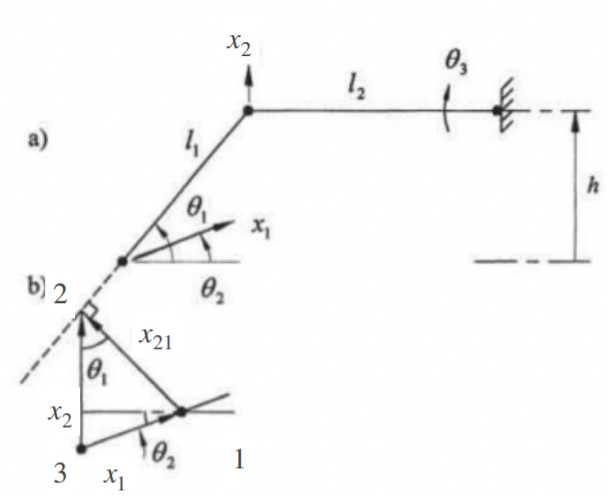
\includegraphics[width=5cm]{two-bar-lever-2}
			\caption{schematic representation (with main design parameters) of a two bar lever with a general input displacement angle $\theta_2$.} \label{fig:ps:twovarlever-2}
		\end{SCfigure}
	
		\paragraph{Soft-spring/stiff-spring attenuation} Considering such flexure system (as in figure \ref{fig:ps:softstiff}) and considering that we have two equivalent springs such that $k_1\ll k_3$, with this implementation we can have a highly linear mechanism (within the elastic range) with extremely large attenuation ($10\,000:1$), however low value of stiffness can stimulate vibrations on the systems.
	
		\paragraph{Lost motion} While dealing with flexure lever mechanisms the parasite stiffness can contribute to the lost motion, so a reduction of theoretical lever ratio.
	
	
	
	
	